\usepackage[italian]{babel}
\usepackage[utf8]{inputenc}
\usepackage{kmath,kerkis}
\usepackage[T1]{fontenc}
\usepackage{color}
\usepackage{hyperref}
\usepackage[absolute, overlay]{textpos}

% fonts
\usefonttheme{serif}
\usefonttheme{structurebold}

% style
\usebackgroundtemplate{
\includegraphics[width=\paperwidth]{images/background}}
\setbeamertemplate{navigation symbols}{}
\definecolor{purple}{RGB}{147,10,0}
\setbeamercolor{structure}{fg=purple}
\setbeamertemplate{items}[circle]
\setbeamercolor*{item}{fg=black}
\setbeamerfont{note page}{size=\footnotesize}

\newcommand{\highlight}[1]{{\color{purple} \emph{#1}}}
\newcommand{\speakernote}[1]{\note[item]{ #1 }}
\newcommand{\ticks}[1]{``#1''}

\title{ Extreme \\ Project Evaluation }

\author{
	Jacopo Franzoi \\
	{\scriptsize jacopo.franzoi@gmail.com }
}

\date{
	Italian Agile Day \\
	Milano, 24 Novembre 2012
}

\begin{document}
	
	\begin{frame}
		\titlepage
		
		\speakernote{ benvenuti, mi presento, 8 anni sviluppo software per mestiere, XP dal 2007. sviluppatore di progetti interni e per clienti, mentore in team per transizione ai Metodi Agili }
		\speakernote{ quinto anno come speaker IAD, riprendo \ticks{\emph{Extreme Release Planning}} @ IAD 2009, in cui ho raccontato come ottenere ed usare un piano di rilascio adottando XP, col \textbf{kick-off} di progetto }
		\speakernote{ la domanda ora è: cosa avviene \textbf{prima} del kick-off? }
	\end{frame}	

	\begin{frame}{Valutazione di Progetti}
		\begin{quote}
			{\small "<{How can you plan a project if you only have a week? [..] You don't have enough time to write a complete set of stories [..] You don't have time to write prototypes so you can estimate the stories from experience}">}
		\end{quote}
		\hfill {\scriptsize K.Beck, Extreme Programming Explained - 1st Edition}

		\begin{itemize}
			\item Scenari
			\begin{itemize}
				\item Budgeting, pre-sales
				\item Studio di fattibilità
				\item Offerta commerciale
			\end{itemize}
		\end{itemize}
		
		\speakernote{ ci viene chiesto di valutare un possibile progetto software. non abbiamo molto tempo per rispondere, ma la risposta deve essere \textbf{indicazione} attendibile. budget per potenziale cliente o cliente esistente, tempi di realizzazione per progetti interni }
		\speakernote{ non possiamo \textbf{permetterci} di dedicare tutto il tempo necessario per pianificare in dettaglio, né per i prototipi per tutti i rischi tecnici }
		\speakernote{ vi racconto \textbf{un modo} di affrontare queste situazioni, partendo da quanto ho imparato applicando XP }
	\end{frame}


	\begin{frame}{Cosa propone XP?}
		\begin{itemize}
			\item Planning in Extreme Programming
			\begin{itemize}
				\item \highlight{Strategia}: esplorazione, commitment, steering
				\item \highlight{Valori}: semplicità, comunicazione, feedback
			\end{itemize}
		\end{itemize}

		\begin{itemize}
			\item E per la \highlight{valutazione} di progetti?
			\begin{itemize}
				\item Granularità grossa (scope, stime)
				\item Esperienza pregressa
				\item Report entro pochi giorni
				\item Planning Game al kick-off
			\end{itemize}
		\end{itemize}
		
		\begin{center}
			\textbf{Esplorazione, Commitment, Reporting}
		\end{center}
		
		\speakernote{ in XP la pianificazione è una \textbf{strategia} in 3 attività: esplorazione (indagine del contesto), commitment (impegno per una soluzione) e steering (aggiustare impegno sulla base dal riscontro) }
		\speakernote{ \textbf{attività} e non fasi: non sequenziali, ma raffinamenti successivi }
		\speakernote{ in XP i \textbf{valori} sottendono alle pratiche. planning: semplicità (2 ruoli, regole semplici, tecniche \ticks{leggere}), comunicazione (evitiamo fraintendimenti, condividiamo gli obiettivi), feedback (adattiamo alla luce di quanto appreso) }
		\speakernote{ affrontiamo il rischio della valutazione. \textbf{granularità} grossa: scope dei temi/storie, scala delle stime (settimane). ci affidiamo a esperienza pregressa: tecnologie, dominio, team. \textbf{timebox} valutazione. planning game d'avvio per \textbf{steering}}
	\end{frame}


	\begin{frame}{Esplorazione: Brainstorming}
		\begin{columns}[T]
		    \begin{column}{.5\textwidth}
				\begin{itemize}
					\item Guida il \highlight{cliente}
					\item Materiale esistente
					\begin{itemize}
						\item Presentazioni
						\item Documentazione
						\item Siti web
					\end{itemize}
				\end{itemize}	

				\begin{itemize}
					\item \textbf{Mappa mentale}
					\begin{itemize}
						\item Idea centrale
						\item Collegamenti
						\item A mano, colori
					\end{itemize}
				\end{itemize}
		    \end{column}
		    \begin{column}{.5\textwidth}
				\hspace*{-0.4cm} 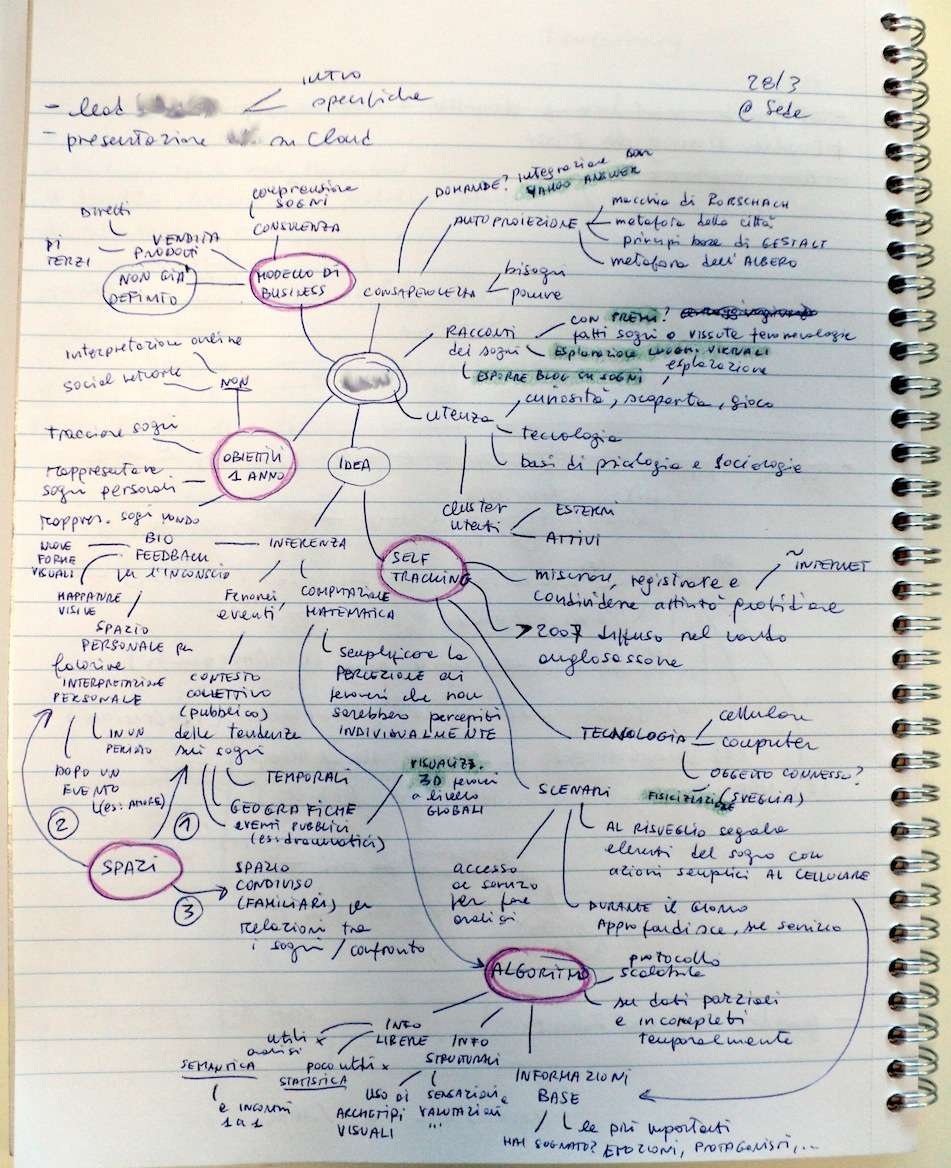
\includegraphics[scale=0.17]{images/mindmap-1}
		    \end{column}
		 \end{columns}
		
		\speakernote{ \textbf{chiacchierata} iniziale, cliente introduce al team. nuovo progetto: presentazione (usata con altri fornitori). rifacimento: website o demo sistema esistente }
		\speakernote{ appunti con mappa mentale: tecnica per \textbf{visualizzare} informazioni. idea centrale, collegamenti tra concetti. a mano, forme, colori.}
		\speakernote{ dominio, fasi e scadenze. appunti: note, dubbi e domande. \textbf{non in dettaglio}, bisogna quindi saper interrompere e rimandare }

	\end{frame}

	\begin{frame}{Esplorazione: Cosa?}

		\begin{columns}[T]
		    \begin{column}{0.6\textwidth}

				\begin{itemize}
					\item Storie, temi
					\item Scadenze, eventi
				\end{itemize}

				\begin{itemize}
					\item \textbf{Piano di rilascio}
					\begin{itemize}
						\item Note, domande
						\item Nessuna stima
					\end{itemize}
					\item \textbf{Modello del dominio}
					\begin{itemize}
						\item Entità, relazioni
						\item Cardinalità
					\end{itemize}
				\end{itemize}
				
			\end{column}
			\begin{column}{0.4\textwidth}
				\hspace*{-0.9cm} 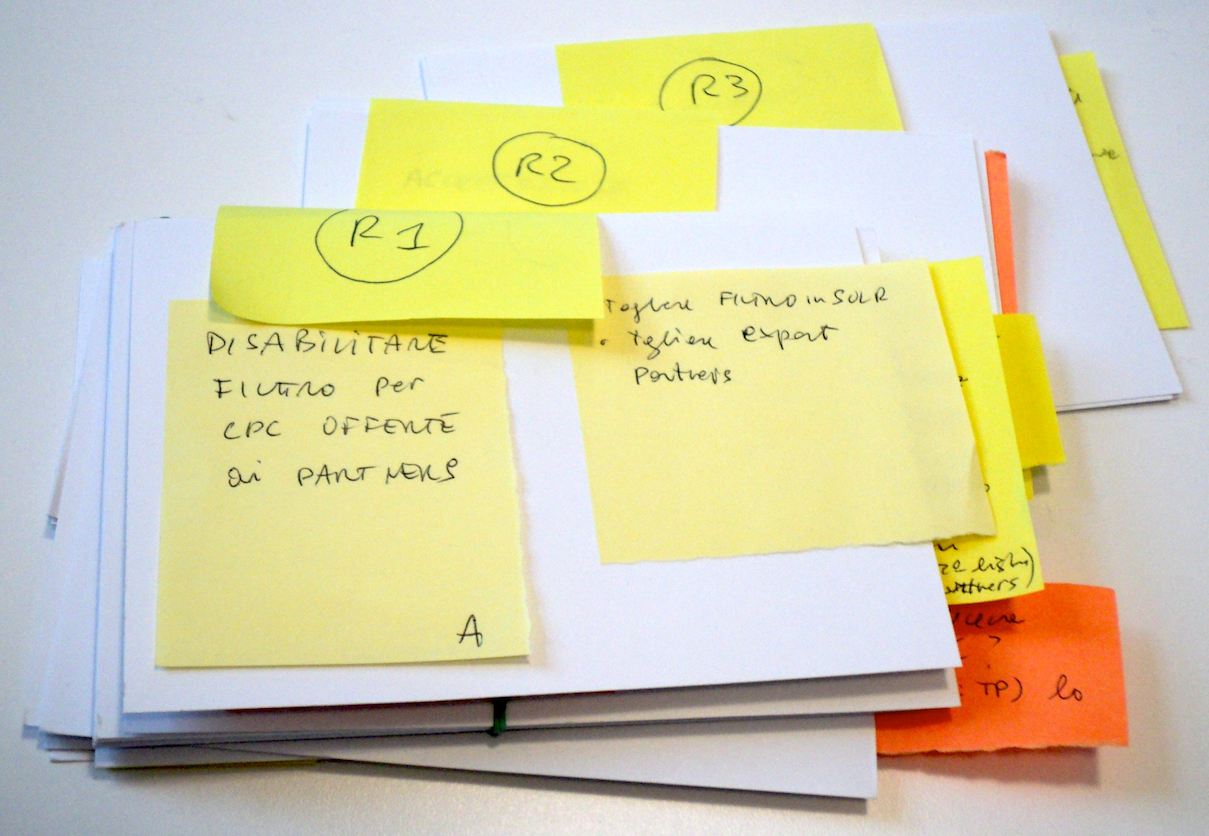
\includegraphics[scale=0.115]{images/stories}
				\\ \vspace*{0.4cm}
				\hspace*{-0.9cm} 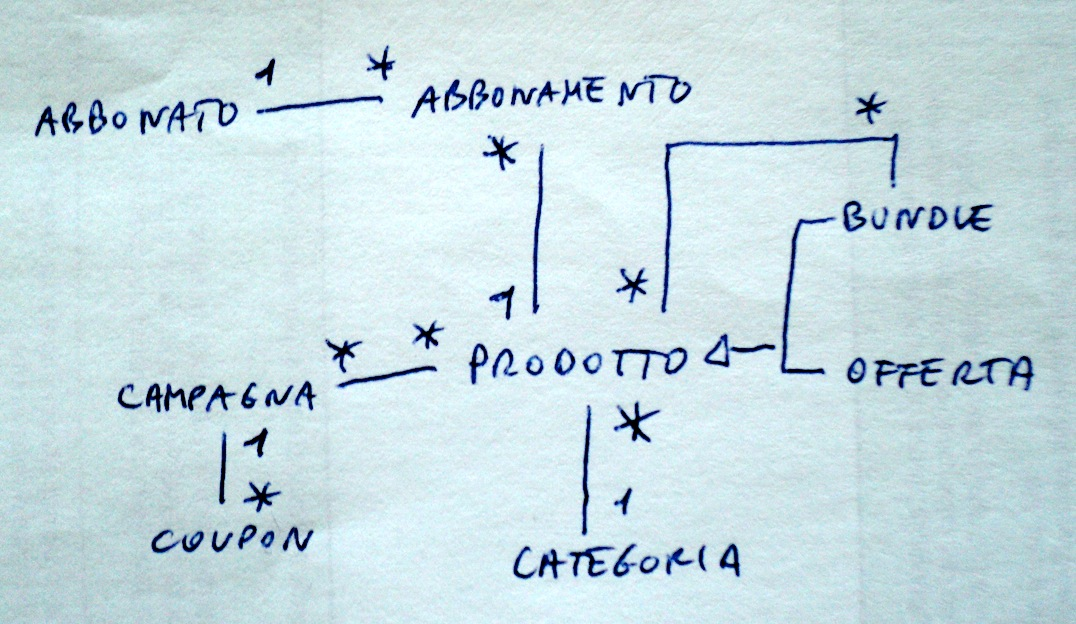
\includegraphics[scale=0.13]{images/domain-1}
			\end{column}
		\end{columns}
		
		\speakernote{ \textbf{analisi}: in XP con user stories. cartoncini scritti a mano, nome, note, domande. granularità grossa (temi), es: aree website, servizi offerti. }
		\speakernote{ indipendenti: \ticks{in che ordine?}, negoziabili: \ticks{facciamo o no?}. \textbf{nessuna stima} perché esplorazione, non commitment. }
		\speakernote{ glossario concetti di dominio, relazioni, cardinalità. obiettivo: \textbf{linguaggio} comune, comprensione, comunicazione. concetti: identità. relazioni: associazione, appartenenza, catalogo. cardinalità: 1, molti, opzionalità}
		\speakernote{ proposta di piano di rilascio: storie \textbf{raggruppate}. criteri: servizi offerti, scadenze ed eventi, rischio. }
		% \speakernote{ \textbf{raffinamenti}. es: split per fotografare rischio/complessità. es: estratto concetto da attributo, cardinalità diventa 0..1 (opzionale). }
	
	\end{frame}

	\begin{frame}{Esplorazione: Come?}
		
		\begin{columns}[T]

		    \begin{column}{.5\textwidth}
				\begin{itemize}

					\item \textbf{Architettura Logica}
					\begin{itemize}
						\item Sistemi
						\item Interconnessioni
						\item Clients (e utenti)
					\end{itemize}
				
					\item \textbf{Hosting}
					\begin{itemize}
						\item In-house, cloud
						\item Pro, staging
					\end{itemize}
				
					\item \textbf{Spikes}
					\begin{itemize}
						\item Prototipi
						\item Time-boxed
					\end{itemize}
				\end{itemize}
			\end{column}
			
			\begin{column}{.5\textwidth}
				\hspace*{-0.6cm} 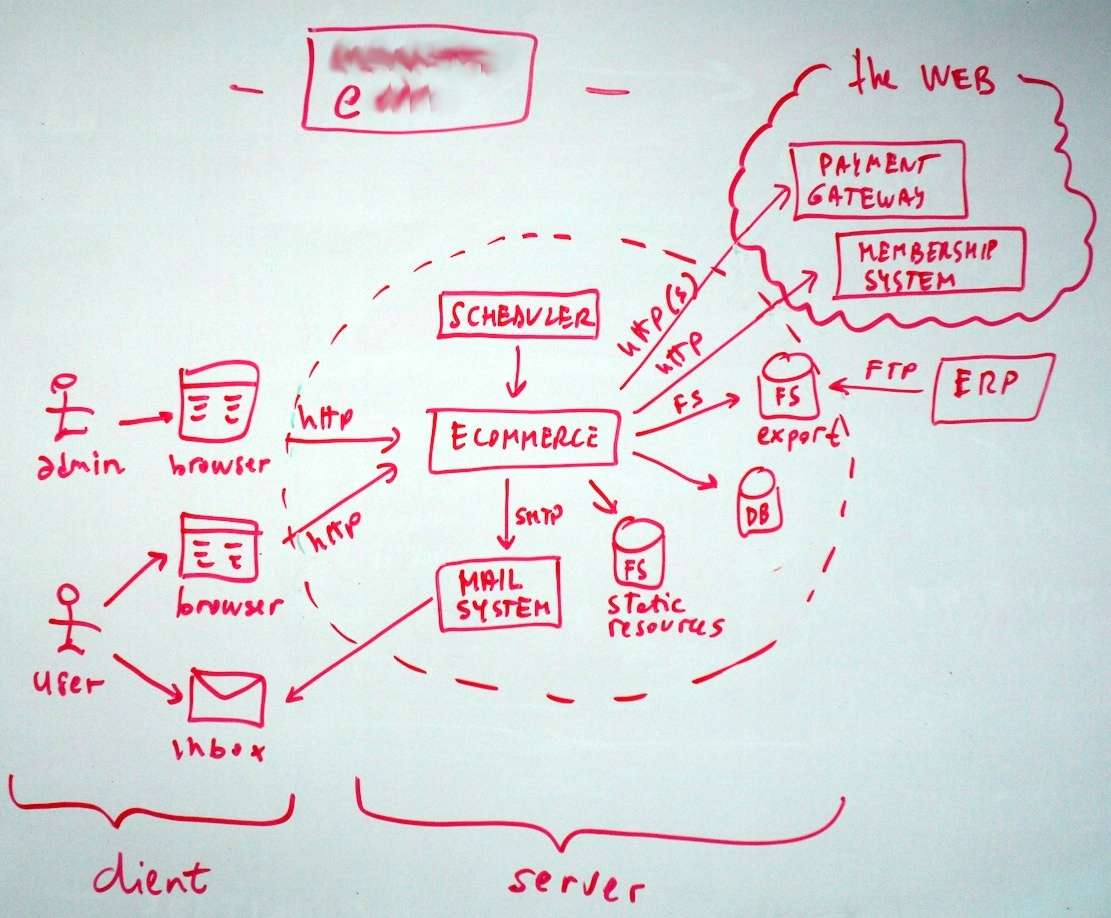
\includegraphics[scale=0.15]{images/architecture-1} \\
				{\scriptsize N.Pryce, TDD of Asynchronous Systems}
			\end{column}
			
		\end{columns}
		
		\speakernote{ \textbf{design} di sistema: in XP architettura evolve con lo sviluppo. individuare rischi: sistemi esterni, tecnologie. delle tante \ticks{viste} con cui descrivere architettura, scegliamo \ticks{componenti e connettori}: quali sistemi (componenti logici), come parlano (protocolli), come accedono gli utenti (client) }
		\speakernote{ requisiti di hosting: server-farm \textbf{esistente}? su cloud? ambiente di collaudo? procedure di collaudo? in assenza di vincoli, proposta da \textbf{esperienza} pregressa }
		\speakernote{ spikes per rischi: sistemi esterni, tecnologie. \textbf{prototipi} usa e getta, versionati per consultazione. timebox per maggiore \textbf{focus} }

	\end{frame}

	\begin{frame}{Commitment: Stima}
		
		\begin{columns}[T]
		   \begin{column}{.5\textwidth}

			\begin{itemize}
				\item Complessità
				\begin{itemize}
					\item Minima, 50\%
					\item Massima, 90\%
					\item Tempo ideale
				\end{itemize}
				\item Incertezza
				\begin{itemize}
					\item Buffer ($ \sigma $)
				\end{itemize}
			\end{itemize}

			\begin{itemize}
				\item \textbf{Effort}
				\begin{itemize}
					\item Minima + Buffer
				\end{itemize}
			\end{itemize}

		   \end{column}
		   \begin{column}{.5\textwidth}
				\vspace*{-0.4cm}
				\hspace*{-0.8cm} 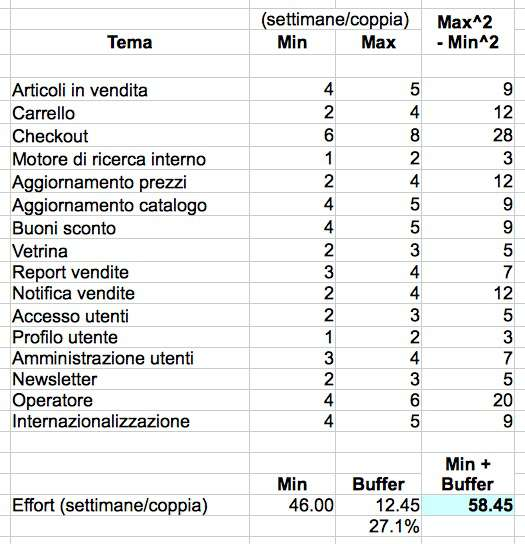
\includegraphics[scale=0.28]{images/effort} \\
				\vspace*{0.2cm}
				{\small $ \sigma = \sqrt[2] { \sum \left ( max^{2} - min^{2} \right ) } $} \\
				{\scriptsize M.Cohn, Agile Estimating and Planning}
		   \end{column}
		\end{columns}
		
		\speakernote{ abbiamo capito i desiderata del cliente e abbiamo una supposizione per come realizzarli. ora dobbiamo capire se sia sostenibile: il \textbf{team} fornisce stime per temi/storie. supposizione, non promessa }
		\speakernote{ dobbiamo gestire \textbf{incertezza}: 1) unità di misura a granularità grossa, settimane/coppia ideali (pair programming) 2) due livelli di confidenza, probabilità di riuscire: 50\% (minima, tutto va liscio e abbiamo esperienza pregressa), 90\% (massima, emergono complessità) }
		\speakernote{ indicatore \textbf{statistico}, buffer derivato dalla deviazione standard: \emph{radice della somma degli scarti quadratici} }
		\speakernote{ sommando questo buffer alla stima al 50\% otteniamo l'effort, indicazione di \textbf{quanto lavoro} ci sia da fare }
		
	\end{frame}

	\begin{frame}{Commitment: Piano di Rilascio}

		\begin{columns}[T]
		    \begin{column}{.55\textwidth}

				\begin{itemize}
					\item Composizione team
					\begin{itemize}
						\item Coppie, coach
						\item Tempo reale
						\item Velocità (prevista)
					\end{itemize}
				\end{itemize}

				\begin{itemize}
					\item \textbf{Elapsed}
					\begin{itemize}
						\item Originale
						\item Per il business
					\end{itemize}
				\end{itemize}
				
				\begin{itemize}
					\item \small{Precisione vs. accuratezza}
				\end{itemize}
		
	    	\end{column}
	
		    \begin{column}{.45\textwidth}
				\hspace*{-0.3cm} 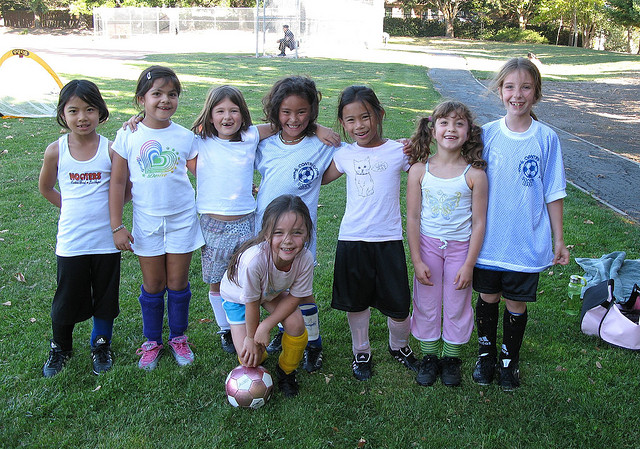
\includegraphics[scale=0.55]{images/team}
				\\ \vspace*{0.2cm}
				\hspace*{-0.5cm} 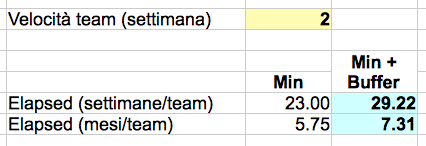
\includegraphics[scale=0.34]{images/elapsed}
		    \end{column}
		\end{columns}

		\vspace*{0.5cm}
		
		{\footnotesize \highlight{\href{http://www.flickr.com/photos/kimberlyjennery/1210060984/}{http://www.flickr.com/photos/kimberlyjennery/1210060984/}}}
		
		\speakernote{ individuiamo la velocità del team. quante coppie, \textbf{rapporto} tra tempo ideale e tempo reale: avvio progetto, overhead processo - non errore di stima! }
		\speakernote{ otteniamo \textbf{quanto tempo} occorre per realizzare il progetto. a seconda dell'interlocutore, la esprimiamo con unità di misura diverse. internamente: \ticks{quante iterazioni?} in settimane/team. per il business: \ticks{quando finisce?} in mesi/team }
		\speakernote{ in fase di valutazione è indicazione, che diventerà eventualmente una \textbf{data} al kick-off di progetto: da quando si parte, aggiunte ferie e varie. es: 8 mesi = gen - ago}

	\end{frame}
	
	\begin{frame}{Commitment: Costi}
		
		\begin{columns}[T]
		    \begin{column}{.5\textwidth}
			
				\begin{itemize}
					\item Hosting
						\begin{itemize}
							\item Previsione
						\end{itemize}
					\item Servizi
					\begin{itemize}
						\item Monitoring
						\item Version control
						\item Mailing
					\end{itemize}
				\end{itemize}
				
				\vspace*{0.2cm}
				\hspace*{0.5cm} 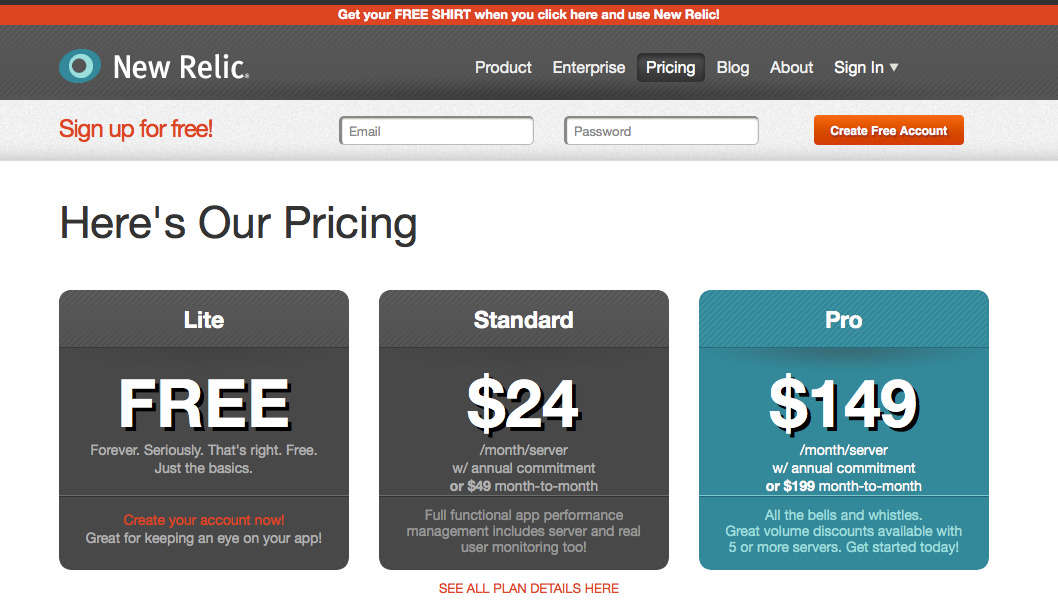
\includegraphics[scale=0.14]{images/costs-3}
    		\end{column}

	    \begin{column}{.5\textwidth}
			\hspace*{-0.8cm} 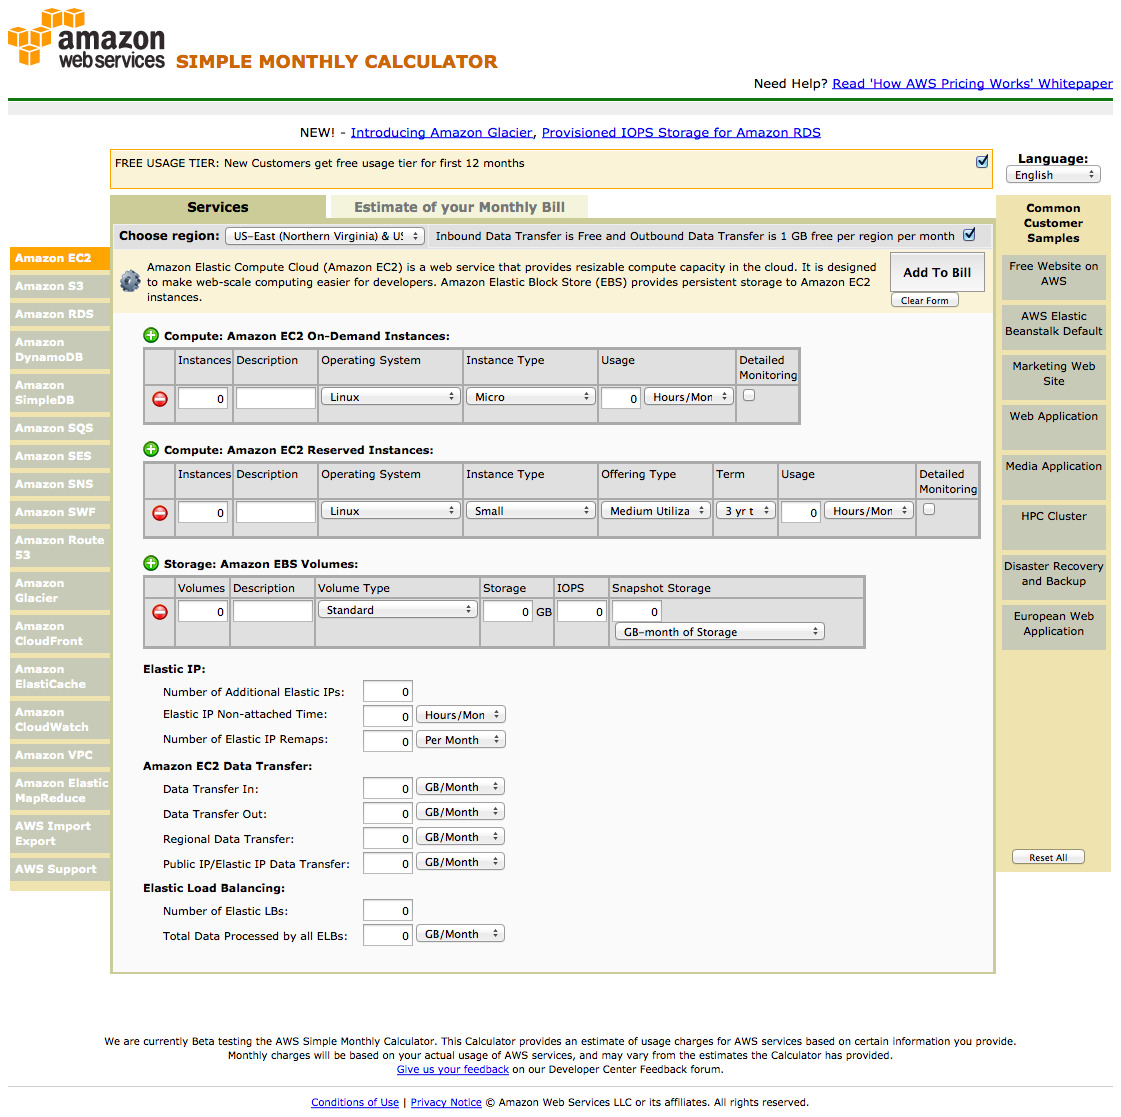
\includegraphics[scale=0.13]{images/costs-1}
			\\ \vspace*{-1cm}
			\hspace*{0.2cm} 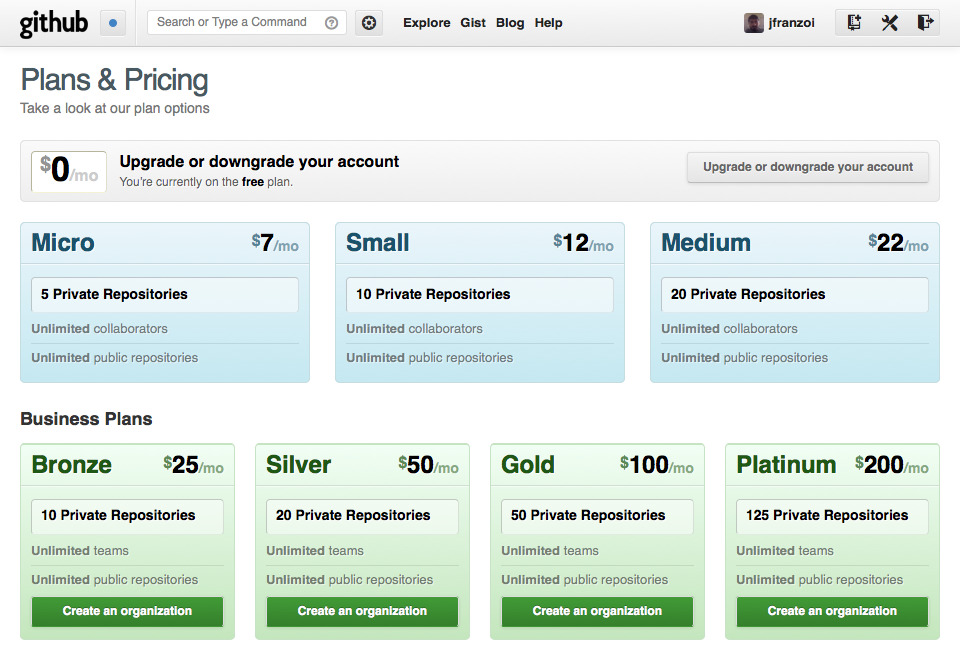
\includegraphics[scale=0.15]{images/costs-2}			
		    \end{column}
		\end{columns}
		
		\speakernote{ ci siamo quasi, ultima indicazione utile: costi di hosting, come previsione per ambienti di produzione e staging. ad esempio usando il calcolatore on-line del servizio di cloud. è la parte \textbf{meno sotto controllo}, dipenderà da architettura e dimensionamento ambienti }
		\speakernote{ anche servizi per l'esercizio e il monitoraggio, ma \textbf{non indispensabili}. indicazione da progetti passati }

	\end{frame}
	
	\begin{frame}{Reporting: Non un \emph{contratto}!}
		\begin{itemize}
			\item \textbf{Introduzione}
			\begin{itemize}
				\item Il team, il cliente
				\item Date incontri
			\end{itemize}

			\item \textbf{Piano di rilascio}
			\begin{itemize}
				\item Narrativa, modello del dominio
				\item Rilasci, temi, composizione team
				\item Tabelle riassuntive: effort, elapsed
			\end{itemize}

			\item \textbf{Soluzione tecnica}
			\begin{itemize}
				\item Architettura logica, hosting
			\end{itemize}

			\item \textbf{Costi}
			\begin{itemize}
				\item Hosting, servizi
				\item Tabella riassuntiva: esercizio
			\end{itemize}
		\end{itemize}
		
		\speakernote{ infine, un \textbf{riassunto} di quanto raccolto. per clienti: un documento, internamente: pagina sulla wiki o spreadsheet condiviso. ecco una \textbf{traccia} }
		\speakernote{ \textbf{1)} presentazione: chi scrive (team), date incontri con il cliente. \textbf{2)} valutazione: narrativa del progetto, usando i concetti di dominio condivisi. modello del dominio come riassunto. narrativa dei rilasci: scope, obiettivi. per ogni rilascio, elenco temi, con note e domande aperte. (eventuale spiegazione come si stima). composizione team. tabelle riassuntive effort (ordine grandezza progetto) ed elapsed (tempo previsto a realizzarlo). \textbf{3)} soluzione tecnica: architettura logica, integrazione sistemi esistenti. vincoli di hosting. \textbf{4)} costi: hosting e servizi a supporto dell'esercizio }
		\speakernote{ mancano \textbf{costi di sviluppo}: non è un contratto, bastano effort e composizione team }
	\end{frame}
	
	\begin{frame}{Sì, ma...}
		\begin{itemize}
			\item \highlight{Che fine hanno fatto le persone?}
				\begin{itemize}
					\item Feedback: cliente, team
					\item Stakeholders: committenti, azienda
				\end{itemize}
			\item \highlight{Per prodotti e progetti interni?}
				\begin{itemize}
					\item Hosting, servizi: standard aziendali
					\item Focus su effort ed elapsed
				\end{itemize}
			\item \highlight{Chi paga per questa valutazione?}
				\begin{itemize}
					\item Preventivo (fornitore)
					\item Kick-start (cliente)
				\end{itemize}
		\end{itemize}
		
		\speakernote{ ecco alcuni \textbf{dubbi} che possono sorgere, e \textbf{obiezioni} che mi sono state fatte }
		\speakernote{ non si sono viste \textbf{abbastanza persone}? fondamentali, raffinamenti successivi dopo feedback del team con tutti gli stakeholders (cliente, tecnici): priorità di business, vincoli tecnici }
		\speakernote{ prodotti e progetti interni, \textbf{senza cliente}? ho cercato di mostrare differenze, ma cliente c'è sempre. alcune cose non si applicano, costi sviluppo già noti, standard per hosting e servizi. info principale sono effort e elapsed dato il team di sviluppo }
		\speakernote{ questa valutazione è un \textbf{investimento}, deve esserci una copertura economica. fornitore, se preventivo per cliente potenziale. cliente, formula del kick-start di 2-5 giorni. in entrambi i casi, timeboxing }
	\end{frame}

	\begin{frame}{Ok, ma...}
		\begin{itemize}
			\item \highlight{Lo prendiamo il progetto?}
				\begin{itemize}
					\item Valutazioni commerciali ed economiche
					\item Collaborazione, controllo ambienti
				\end{itemize}
			\item \highlight{Per il contratto?}
				\begin{itemize}
					\item Rilasci incrementali
					\item Win-win
				\end{itemize}
			\item \highlight{Cosa avviene al kick-off?}
				\begin{itemize}
					\item Planning Game iniziale
					\item Steering: Iteration planning
				\end{itemize}
		\end{itemize}
		
		\speakernote{ alla fine però bisogna \textbf{decidere} se partire. valutazione da entrambe le parti. fornitore valuta rischio rispetto a condizioni economiche. valuta anche rischi dovuti a grado di collaborazione, accesso informazioni e libertà operativa sugli ambienti. (es: buon margine economico, ma accesso in collaudo rigido e poco frequente) }
		\speakernote{ parte difficile: il contratto. \textbf{non solo sintesi} di effort, elapsed e costi, ma garantire rilasci incrementali con accettazione formale. vantaggioso per entrambe le parti: diverse proposte (vedi dopo) }
		\speakernote{ \textbf{arriva ok} per partire: kick-off serve per fare steering. rivisto release planning, convalidato da un iteration planning (scala inferiore) }
	\end{frame}

	\begin{frame}{Cosa Portare a Casa}
		\hspace*{-0.5cm} 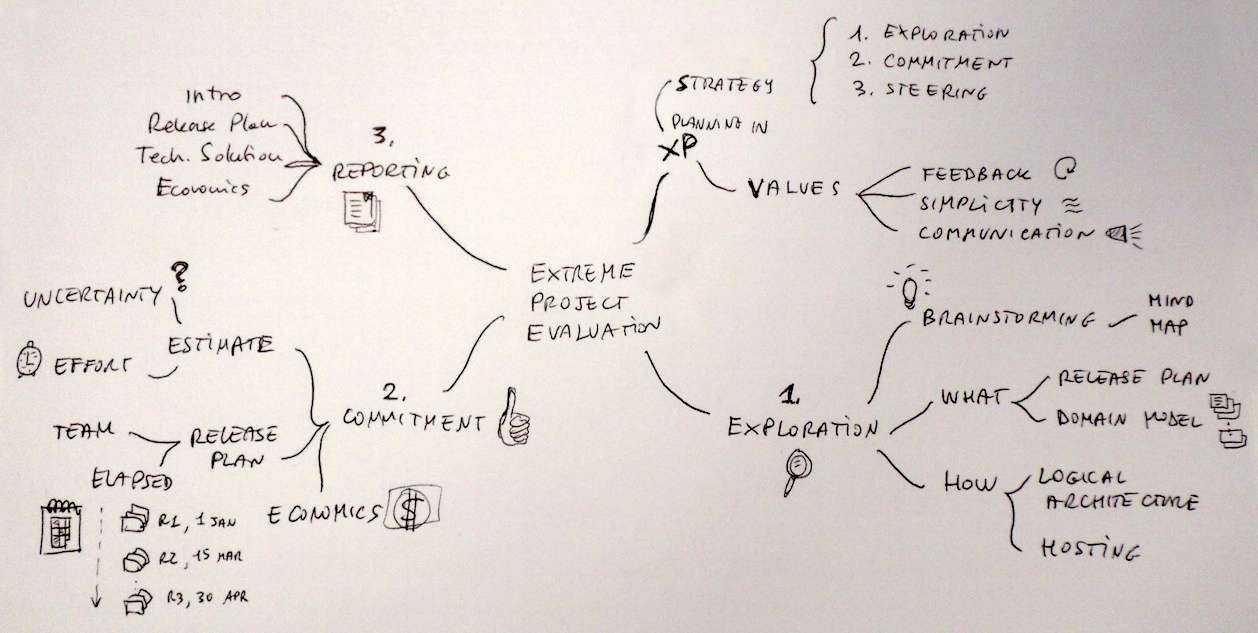
\includegraphics[scale=0.26]{images/takeaway}
		
		\speakernote{ ho messo insieme \textbf{tanti temi}, ciascuno meritava più tempo. con questa panoramica spero di avervi lasciato qualcosa da portare a casa }
		\speakernote{ una \textbf{strategia} per valutare progetti software: esplorazione, commitment e steering. quali valori vi stanno dietro. (di fatto, un'introduzione ad XP) }
		\speakernote{ alcune tecniche per \textbf{esplorare} in modo efficace: mappe mentali per il brain-storming, analisi fatta con user stories e modelli del dominio, per ottenere un piano di rilascio. una prospettiva per descrivere l'architettura logica del sistema }
		\speakernote{ tecniche per \textbf{gestire} incertezza e rischio nelle stime dell'effort, così da ottenere un elapsed che porti ad un piano operativo }
		\speakernote{ infine, una \textbf{traccia} di quanto condividere, per alimentare un eventuale accordo commerciale }
	\end{frame}
	
	\begin{frame}{Per Approfondire}
		\begin{columns}[T]
		    \begin{column}{.8\textwidth}
			
				\begin{itemize}	
					\item \textbf{Pianificazione e valori in XP}
						\begin{itemize}
							\item {\small Kent Beck \highlight{Extreme Programming Explained - 1st ed}}
						\end{itemize}

					\item \textbf{Stima e incertezza}
						\begin{itemize}
							\item {\small Mike Cohn \highlight{Agile Estimating and Planning}}
						\end{itemize}

					\item \textbf{Architettura logica}
						\begin{itemize}
							\item {\small Nat Pryce \highlight{\href{http://www.natpryce.com/articles/000755.html}{Test-Driven Development of Asynchronous Systems}}}
						\end{itemize}

					\item \textbf{Contratti}
						\begin{itemize}
							\item {\small Peter Stevens \highlight{\href{http://agilesoftwaredevelopment.com/blog/peterstev/10-agile-contracts}{10 Contracts for your next Agile Software Project}}}
						\end{itemize}
				\end{itemize}
			\end{column}
			\begin{column}{.2\textwidth}
				\vspace*{-0.4cm}
				\hspace*{0.05cm} 
\includegraphics[scale=0.09]{images/book-1} \\
				\vspace*{0.05cm}
				\hspace*{0.07cm} 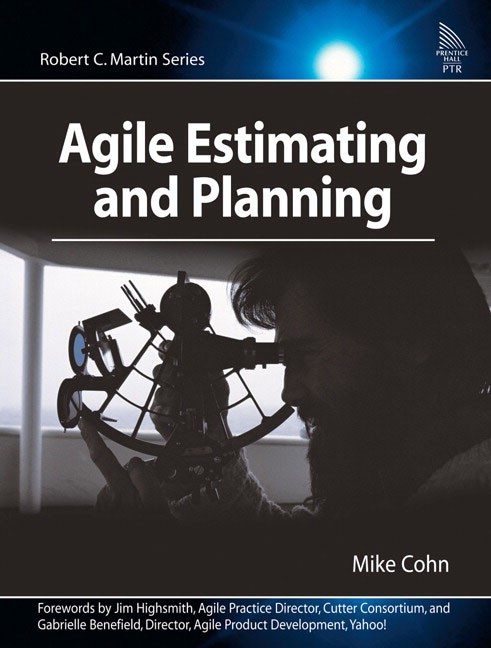
\includegraphics[scale=0.09]{images/book-2} \\
				\vspace*{0.05cm}
				\hspace*{0.35cm} 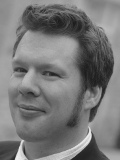
\includegraphics[scale=0.3]{images/book-3} \\
				\vspace*{0.05cm}
				\hspace*{0.1cm} 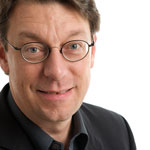
\includegraphics[scale=0.4]{images/book-4}
		    \end{column}
		\end{columns}
		
		\speakernote{ per approfondire, il libro bianco resta il punto di \textbf{riferimento} da cui partire. valori, principi e pratiche. descrizione precisa dei ruoli e delle regole del \ticks{gioco della pianificazione} }
		\speakernote{ \textbf{analisi statistica} che ho mostrato è presa dal libro di Cohn, scritto in chiave Scrum. contiene anche distinzione tra storia, tema ed epica }
		\speakernote{ la prospettiva e la \textbf{notazione} per l'architettura logica dei sistemi è presa da Pryce, che le usa nelle sue presentazioni. per il concetto di \ticks{viste} consiglio \ticks{\emph{Documenting Software Architectures: Views and Beyond - 2nd ed}} di Paul Clemens }
		\speakernote{ per il tema contratti, dopo una \textbf{domanda allo scorso IAD}, ho riportato sul mio blog personale alcuni link, tra cui un articolo di Peter Stevens che ha ispirato una presentazione del Milano XPUG}
	\end{frame}
	
	\begin{frame}{E questo è tutto, gente!}
		
		\begin{itemize}
			\item \textbf{Un grazie a}
			\begin{itemize}
				\item Team \emph{Orione} @ XPeppers
				\item Team \emph{Nimbus} @ 7Pixel
				\item Matteo Vaccari e Davide Varvello
			\end{itemize}
		\end{itemize}
		
		\begin{itemize}
			\item \textbf{Contatti}
				\begin{itemize}
					\item \highlight{ jacopo.franzoi@gmail.com }
					\item \highlight{  \href{http://jacopo.franzoi.googlepages.com/}{http://jacopo.franzoi.googlepages.com} }
					\item \highlight{  \href{http://jfranzoi.wordpress.com/}{http://jfranzoi.wordpress.com} }
				\end{itemize}
		\end{itemize}

	\end{frame}
	
	% \begin{frame}{Esempi: Mappa Mentale}
	% 	\begin{columns}[T]
	% 	    \begin{column}{.5\textwidth}
	% 			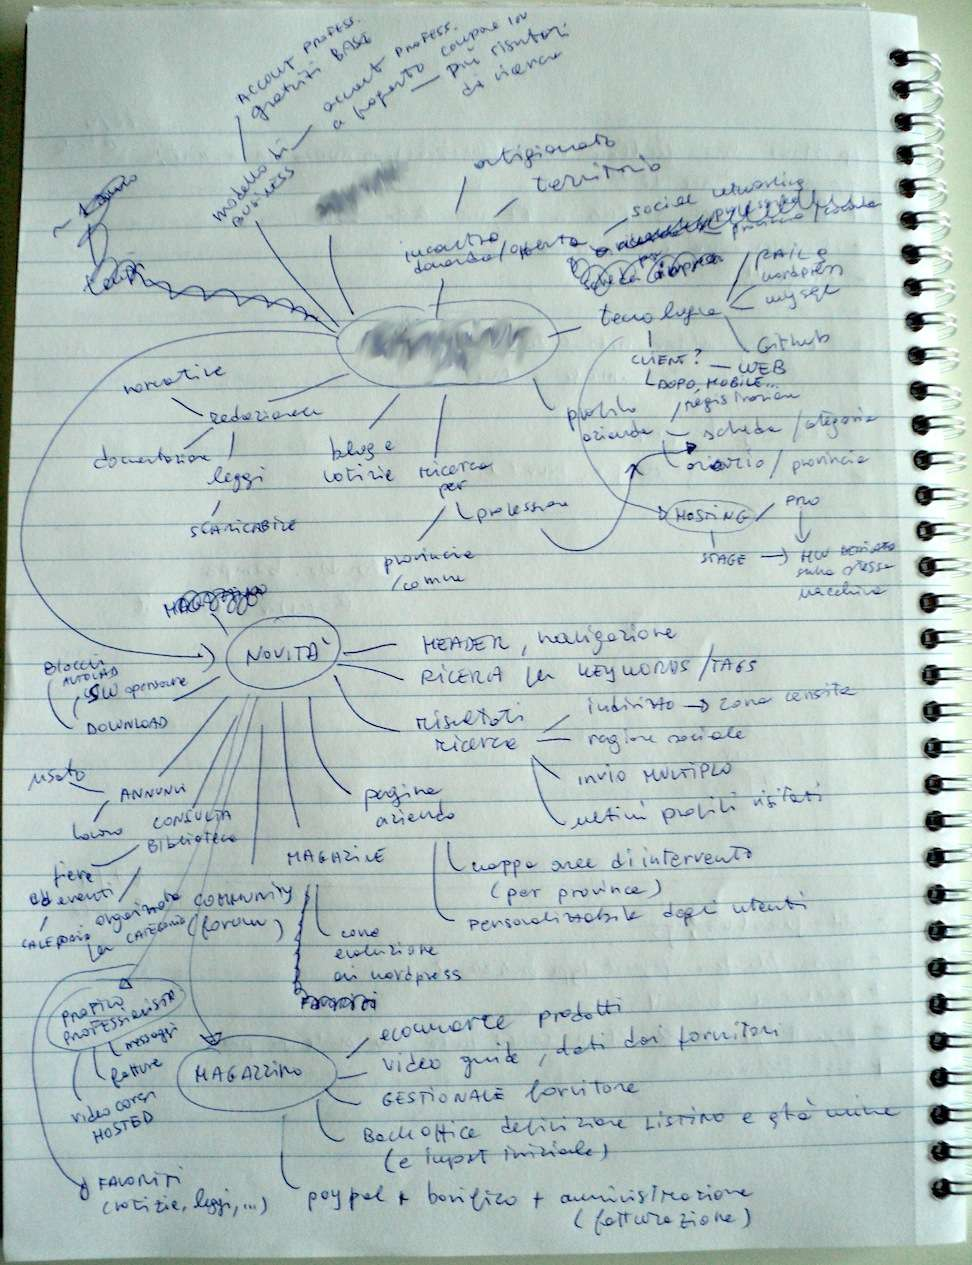
\includegraphics[scale=0.16]{images/mindmap-3}
	% 	    \end{column}
	% 	    \begin{column}{.5\textwidth}
	% 			\hspace*{-0.4cm} 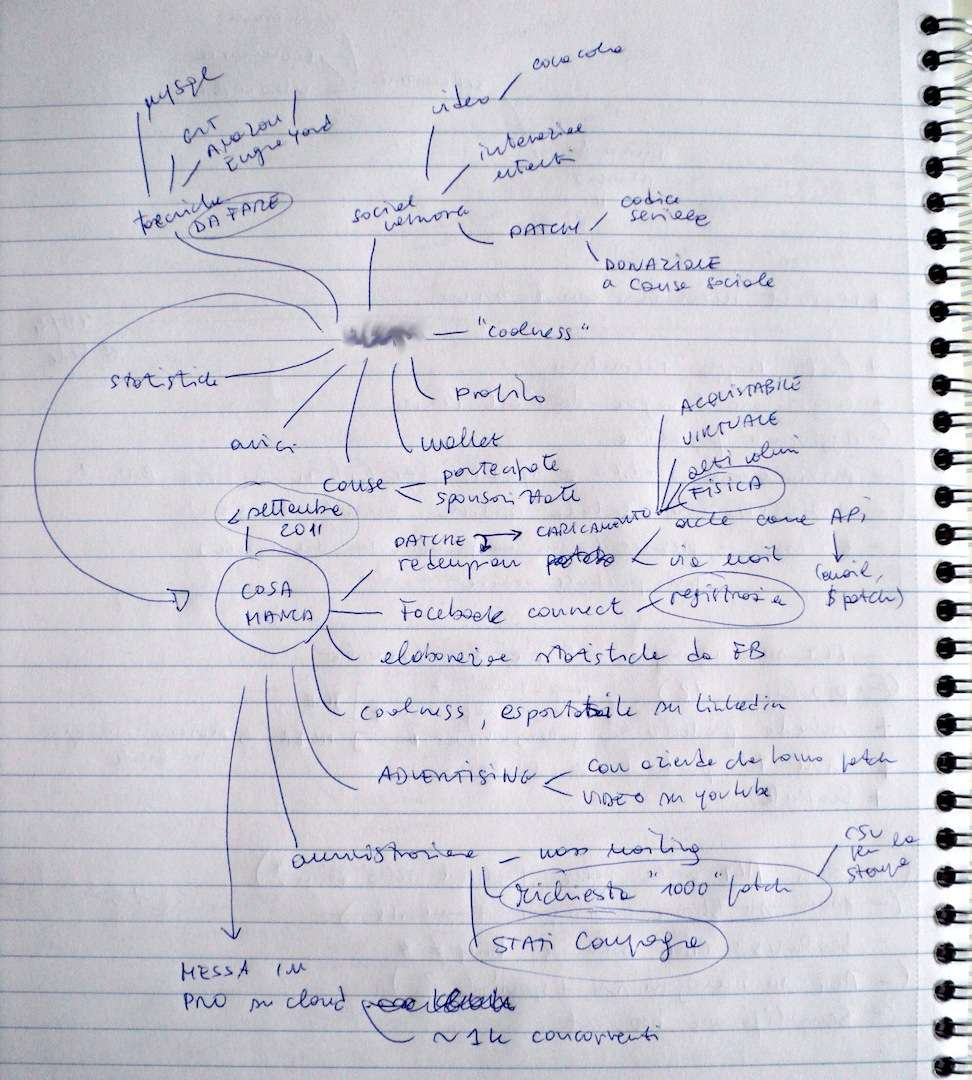
\includegraphics[scale=0.17]{images/mindmap-2}
	% 	    \end{column}
	% 	 \end{columns}
	% \end{frame}
	% 
	% \begin{frame}{Esempi: Modello del Dominio}
	% 	\begin{columns}[T]
	% 	    \begin{column}{.5\textwidth}
	% 			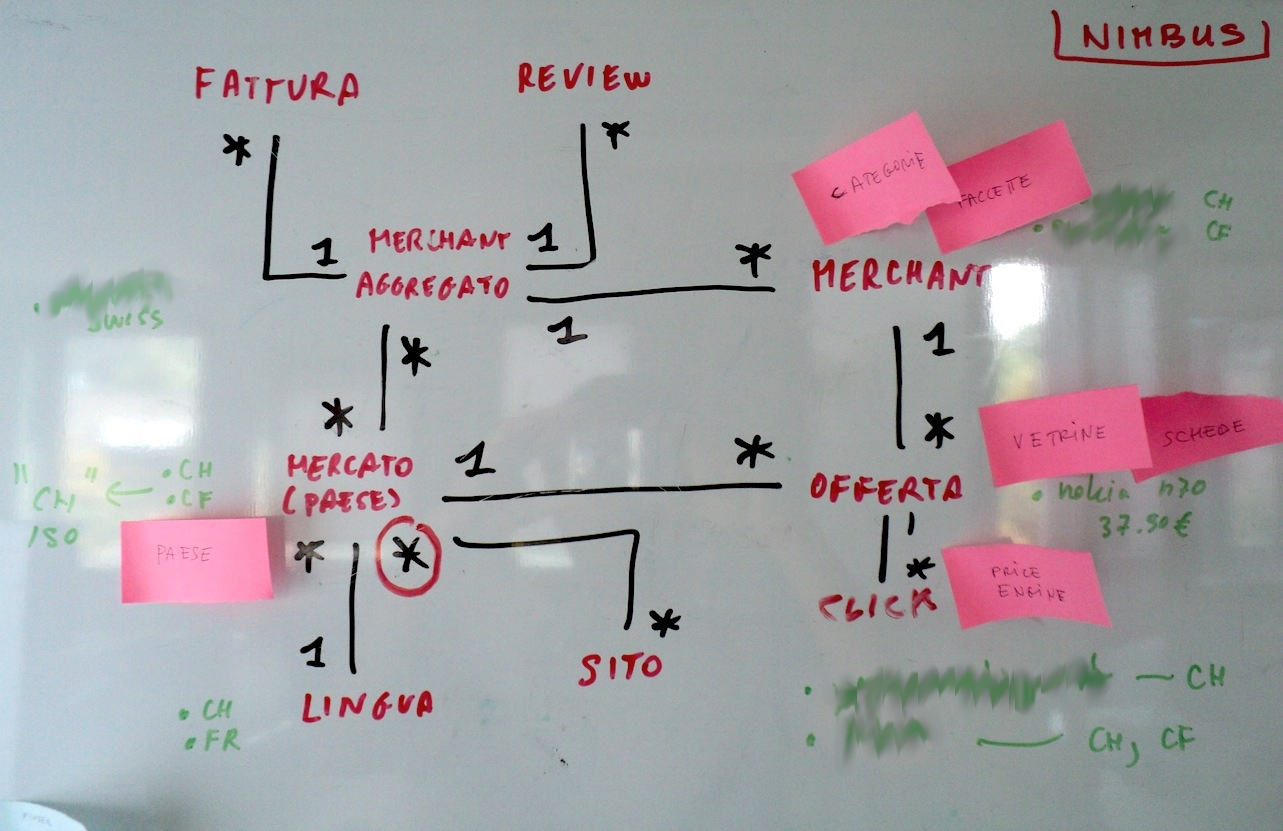
\includegraphics[scale=0.12]{images/domain-2}
	% 			\\ \vspace*{0.4cm}
	% 			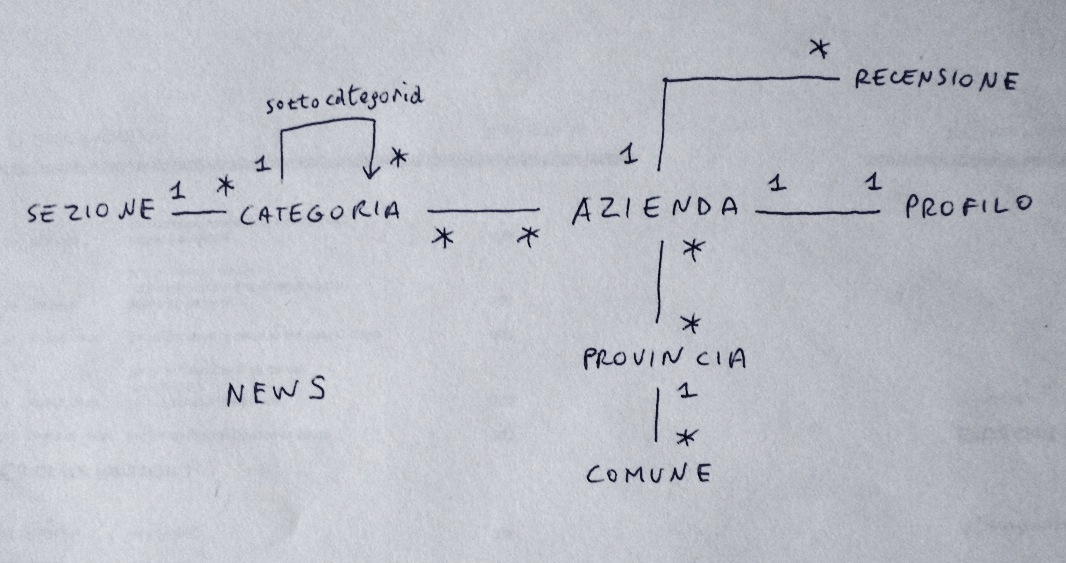
\includegraphics[scale=0.15]{images/domain-4}
	% 	    \end{column}
	% 	    \begin{column}{.5\textwidth}
	% 			\vspace*{0.3cm}
	% 			\hspace*{-0.3cm} 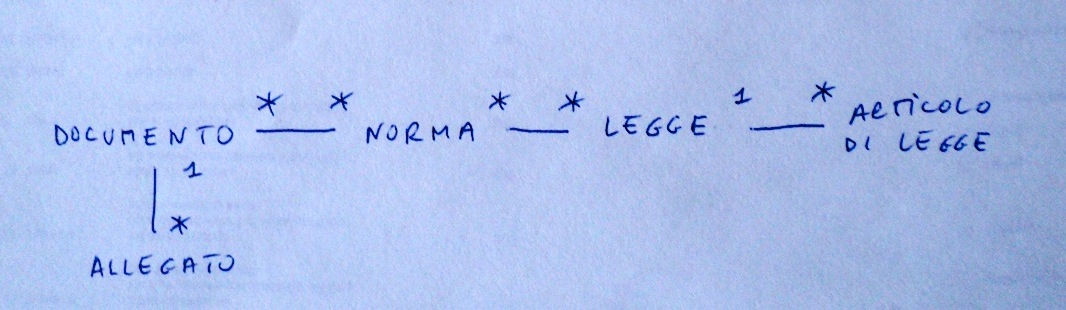
\includegraphics[scale=0.15]{images/domain-5}
	% 			\\ \vspace*{0.3cm}
	% 			\hspace*{-0.3cm} 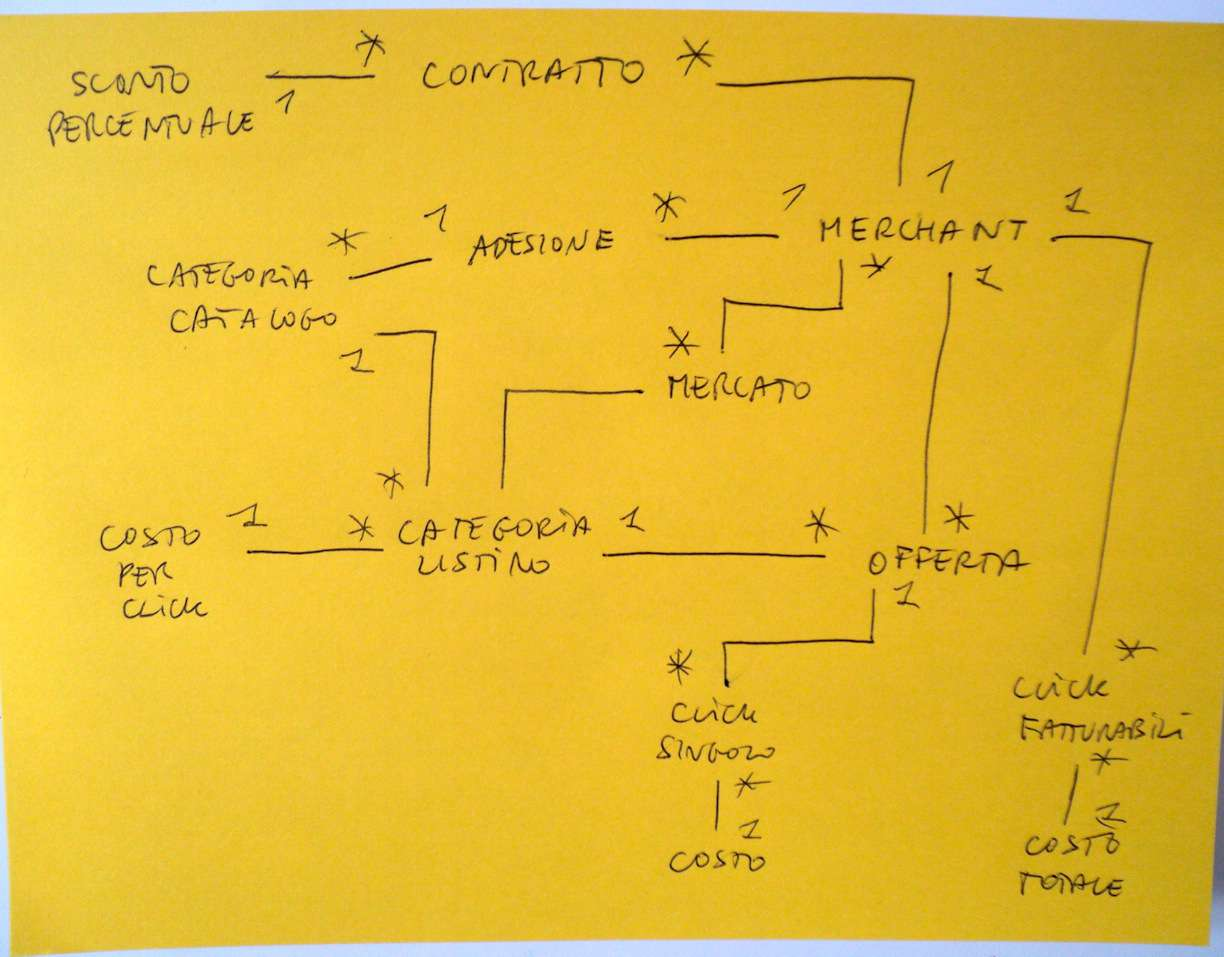
\includegraphics[scale=0.13]{images/domain-3}
	% 	    \end{column}
	% 	 \end{columns}
	% \end{frame}
	% 
	% \begin{frame}{Esempi: Architettura Logica}
	% 	\begin{columns}[T]
	% 	    \begin{column}{.5\textwidth}
	% 			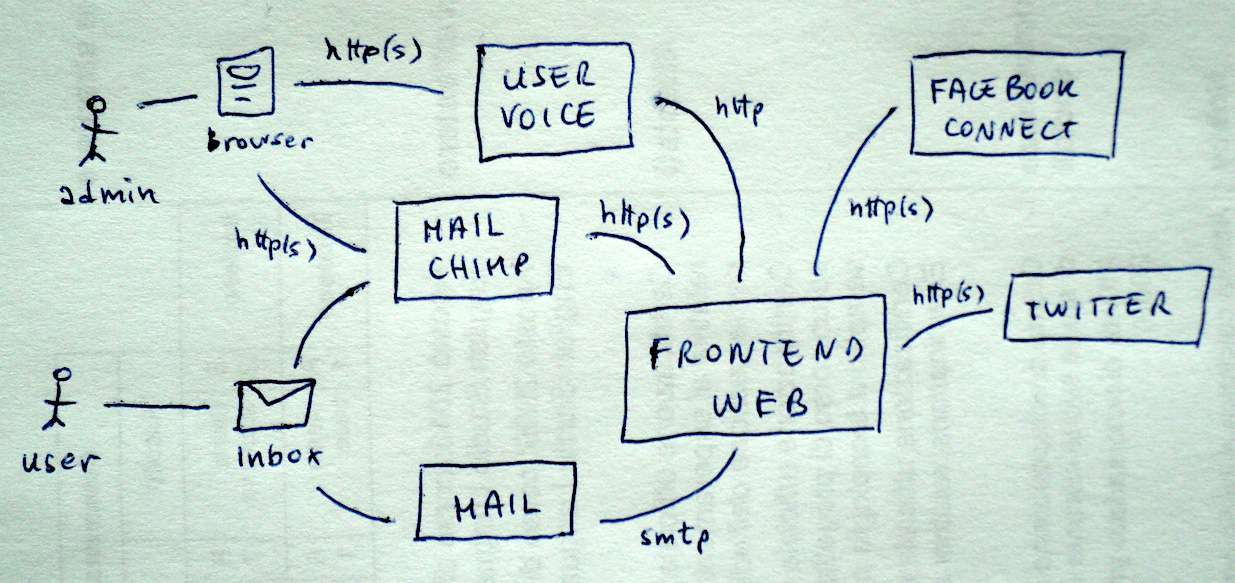
\includegraphics[scale=0.13]{images/architecture-2}
	% 			\\ \vspace*{0.2cm}
	% 			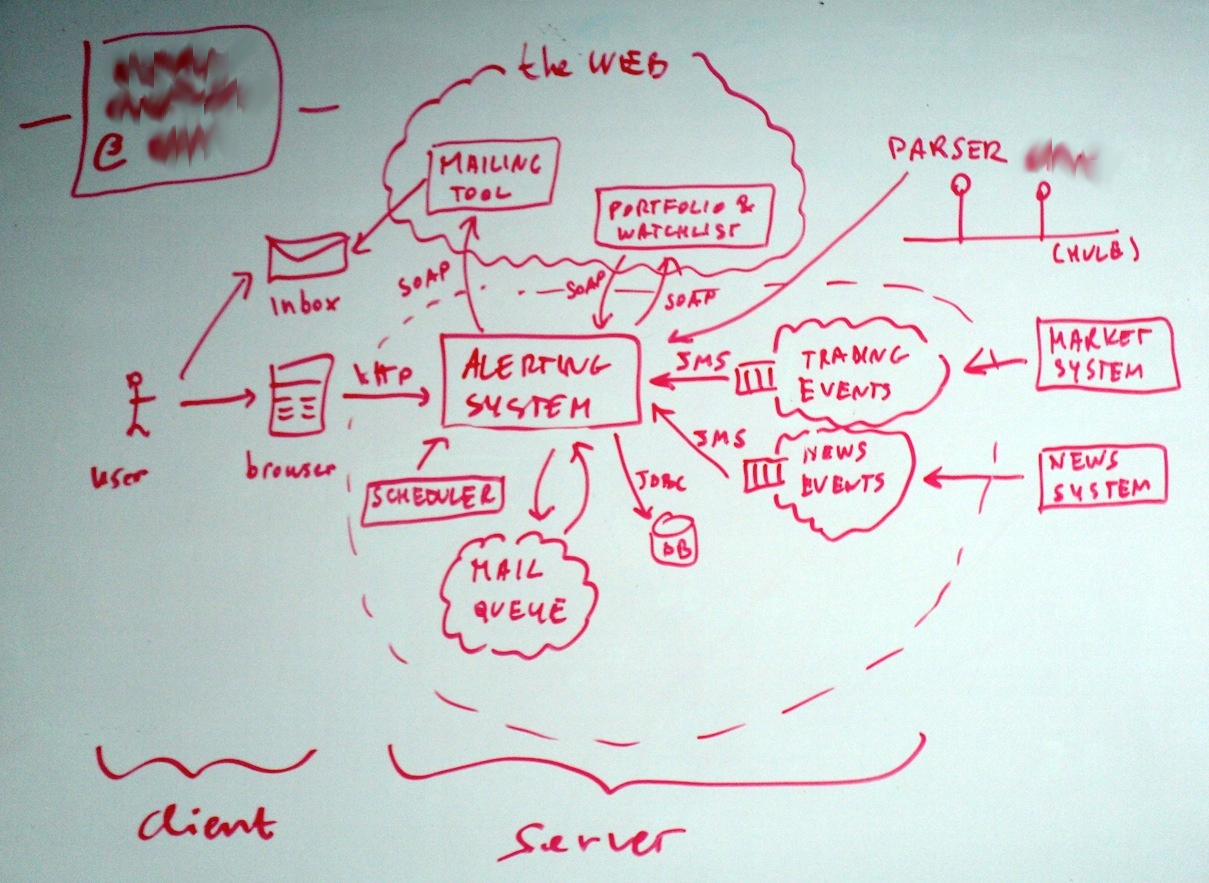
\includegraphics[scale=0.135]{images/architecture-3}
	% 	    \end{column}
	% 	    \begin{column}{.5\textwidth}
	% 			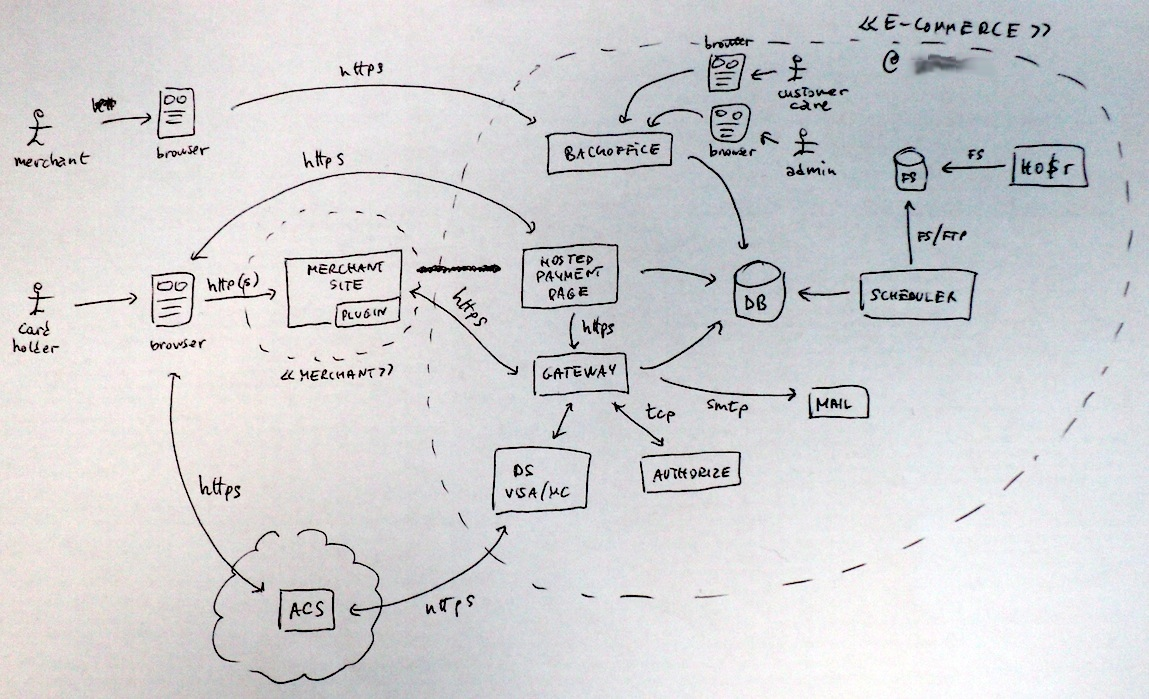
\includegraphics[scale=0.13]{images/architecture-5}
	% 			\\ \vspace*{0.2cm}
	% 			\hspace*{0.2cm} 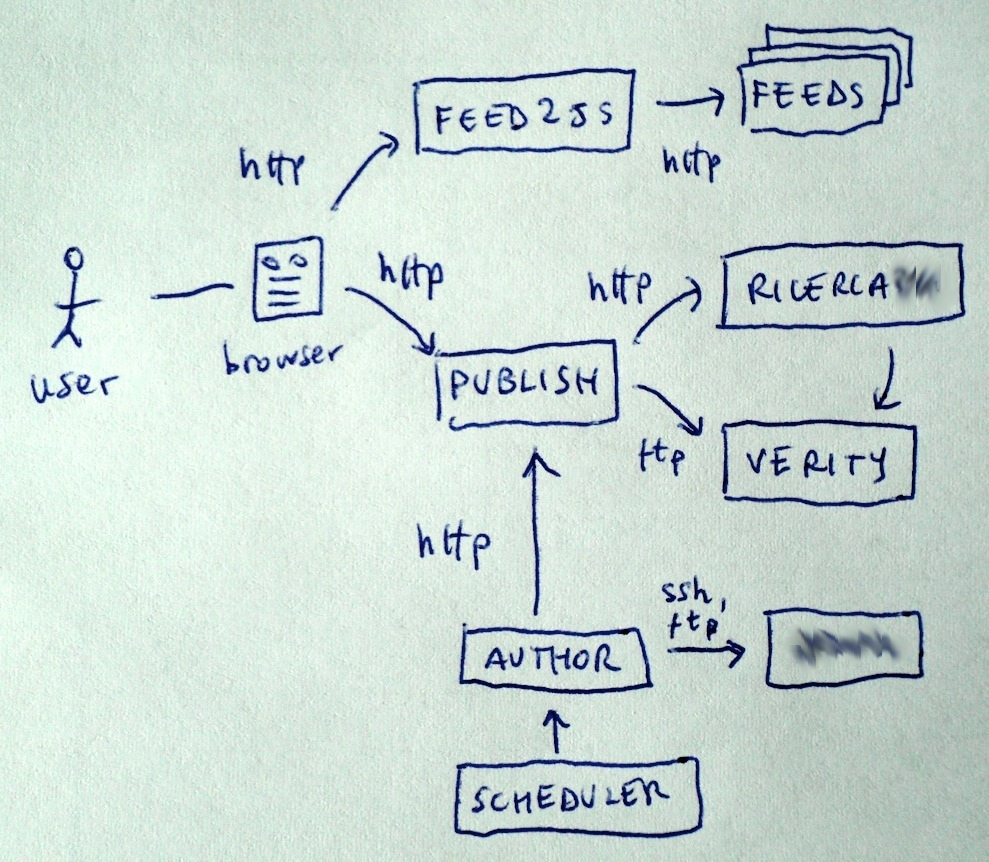
\includegraphics[scale=0.13]{images/architecture-4}
	% 	    \end{column}
	% 	 \end{columns}
	% \end{frame}

\end{document}